\section{Introduction}
In the IRI lab we have two segway robots, Tibi and Dabo show in figure
\ref{fig:Picture of Tibi and Dabo}. Both of them move the same way.
They must incline their body to compensate the wheel reaction torque. We will get deeper
in why this phenomena happens in section \ref{}.

This movement restriction may cause some problems when trying to avoid obstacles,
as for example going through low roof path. Another limitation is the
acceleration that the robot can achieve which is directly related with the inclination
that it's limited to 90 degrees in the best case. Also the amount of uphill
is limited with an additional problem: the safety system stops the robot if 
it detects something near it (in this case the ground).

So we decided to build a prototype of segway robot that could solve this problem by 
controlling it's inclination independently. The chosen robot is inspired in a
\textit{segway hover-board}, similar to the one appearing in Figure \ref{fig:Picture of a commercial 
segway hover-board}. The two wheels are controlled with classic control algorithms and the
inclination of the central body is controlled with a flywheel mechanism that we will
discuss in section \ref{sec: flywheel design}.
\begin{figure}
	\centering
	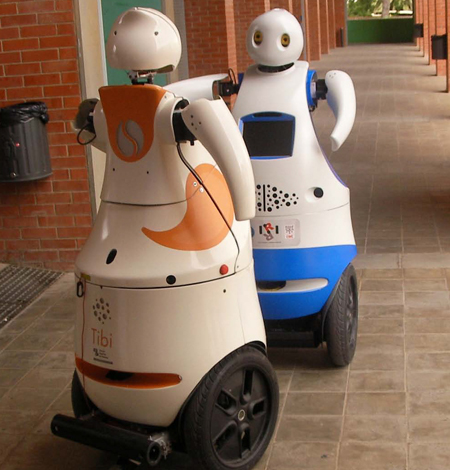
\includegraphics[width=8cm]{img/robots-TIBI-i-DABO-IRI-red.jpg}
	\caption{Picture of Tibi and Dabo, \textit{two segway robots} }
	\label{fig:Picture of Tibi and Dabo}
\end{figure}

\begin{figure}
	\centering
	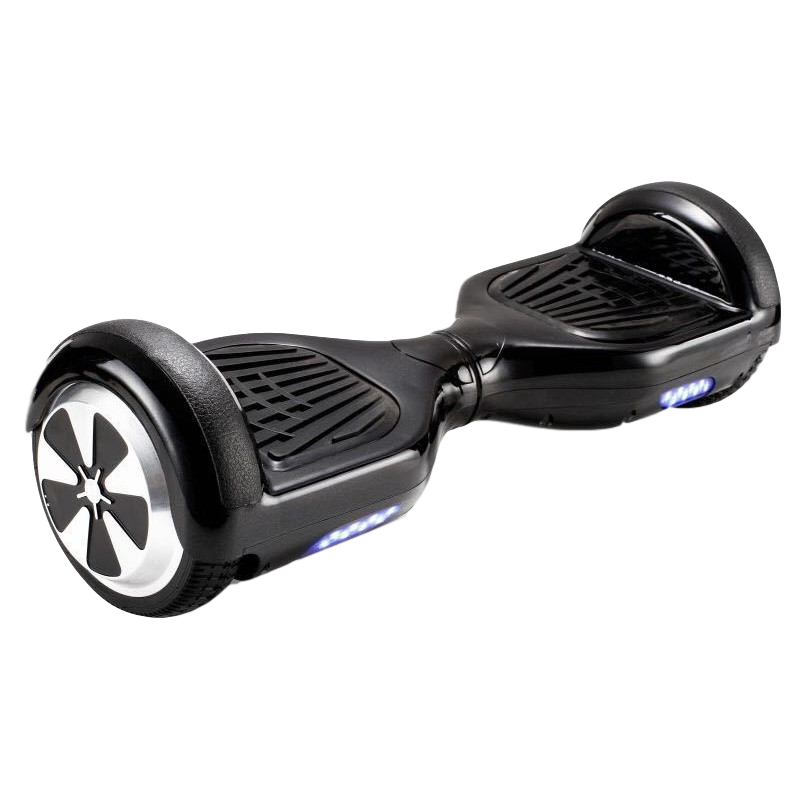
\includegraphics[width=8cm]{img/segway_hoverboard_picture.png}
	\caption{Picture of a commercial \textit{segway hover-board} }
	\label{fig:Picture of a commercial segway hover-board}
\end{figure}
